% =====================================================================
%  第 2 章 辛几何与伪全纯曲线入门 —— ch02a（§2.1–§2.4）
%  页段：PDF 31–62（原书 p.21–52）
%  译者：tr01
% =====================================================================
\chapter{辛几何与伪全纯曲线入门}

% [原文 p.21]
\section{定义与例}

\takeaway{辛形式是满足 $\rd\omega=0$ 且 $\omega^n$ 处处非零的微分 2 形式；余切丛 $T^*M$ 与凯勒流形给出两类基本例子，后者借“复子流形仍是凯勒流形”不断生成新例。}

本节叙述辛流形的定义与基本例子。

\begin{definition}{2.1}
  $2n$ 维流形 $M$ 上的\textbf{辛结构}（symplectic structure）是指 $M$ 上的微分 2 形式 $\omega_M$：它满足 $\rd\omega_M=0$，并且微分 $2n$ 形式 $\omega_M^n$ 处处不为 0。称组 $(M,\omega_M)$ 为\textbf{辛流形}。
\end{definition}

本书中，未加说明时维数一律指实维数，不指复维数。
% [Tutor Note: 此处“$\omega_M^n$ 处处非零”与“$\omega_M$ 非退化”等价，论证只有线性代数一步：在一点取基后 $\omega_M$ 对应反对称矩阵 $A$，$\omega_M^n$ 在该点的值与 $\det A$ 相差一个非零常数因子，故 $\det A\neq 0$ 与 $\omega_M^n\neq 0$ 是同一件事。]

$\omega_M^n\neq 0$ 这一条件，与把 $\omega_M$ 看作切丛（tangent bundle）上的反对称 2 形式时非退化，是等价的。

辛流形最初的重要例子是余切丛（cotangent bundle）。设 $M$ 为流形，$T^*M$ 为其余切丛。在 $T^*M$ 上定义辛结构 $\omega_{T^*M}$。取一点 $x$ 附近 $M$ 的局部坐标 $q_1,\dots,q_n$。此时余切向量空间 $T_x^*M$ 的点可表为 $p_1\rd q_1+\cdots+p_n\rd q_n$。于是可以把 $q_1,\dots,q_n,p_1,\dots,p_n$ 取作 $T^*M$ 的坐标。

\begin{lemma*}{2.2}
  存在 $T^*M$ 上整体定义的微分 2 形式 $\omega_{T^*M}$，它在每点的邻域中、用上述局部坐标可表为 $\omega=\rd q_1\wedge\rd p_1+\cdots+\rd q_n\wedge\rd p_n$。
\end{lemma*}

% [原文 p.22]
\begin{proof}
  要证明的是：微分形式
  \begin{equation}
    \omega = \rd q_1\wedge\rd p_1+\cdots+\rd q_n\wedge\rd p_n \tag{2.1}
  \end{equation}
  不依赖于 $M$ 的局部坐标 $q_1,\dots,q_n$ 的取法。

  设 $\pi\colon T^*M\to M$ 为余切丛的投影，$TT^*M$ 为（视为流形的）$T^*M$ 的切丛。微分 $\pi$ 给出映射 $\rd\pi\colon T_{(x,v)}T^*M\to T_xM$。定义 $T^*M$ 上的微分 1 形式 $\theta$ 为
  \[
    \theta_{(x,v)}(w)=v(\rd\pi(w)).
  \]
  这里 $x\in M$，$v\in T_x^*M$，又 $w\in T_{(x,v)}T^*M$。左边是在点 $(x,v)$ 处把 $w$ 代入 $\theta$ 所得的值。右边说明如下：$\rd\pi(w)$ 是切向量空间 $T_xM$ 的元素；而 $v\in T_x^*M$，$T_x^*M$ 是 $T_xM$ 的对偶向量空间，故实数 $v(\rd\pi(w))$ 确定。称 $\theta$ 为\textbf{基本形式}（fundamental form）。

  稍加审视定义便知 $\theta=p_1\rd q_1+\cdots+p_n\rd q_n$。于是
  \[
    \rd\theta=\rd p_1\wedge\rd q_1+\cdots+\rd p_n\wedge\rd q_n=-\omega.
  \]
  $\theta$ 的定义没有用到坐标，故 $\theta$ 是 $T^*M$ 整体上定义的微分 1 形式。因此其外微分 $\rd\theta$ 也是 $M$ 整体上定义的微分 2 形式，不依赖于 $M$ 的坐标取法。
\end{proof}
% [Tutor Note: 由 $\theta=p_1\rd q_1+\cdots+p_n\rd q_n$ 得到 $\rd\theta=-\omega$，负号源自 $\omega$ 取 $\rd q_i\wedge\rd p_i$ 的顺序；若改取 $\rd p_i\wedge\rd q_i$ 则 $\rd\theta=\omega$。这一符号约定贯穿全书，原书 p.29 的注 2.19 专门讨论过。]

\begin{lemma*}{2.3}
  $(T^*M,\omega_{T^*M})$ 是辛流形。
\end{lemma*}

\begin{proof}
  由式 (2.1) 得 $\rd\omega_{T^*M}=\rd\rd\theta=0$。另一方面，用局部坐标表示时 $\omega_{T^*M}^n=n!\,\rd q_1\wedge\rd p_1\wedge\cdots\wedge\rd q_n\wedge\rd p_n$，故 $\omega_{T^*M}^n$ 决不取 0。
\end{proof}

辛流形的例子还有另一个重要源泉，即凯勒流形。

\begin{definition}{2.4}
  $2n$ 维流形 $M$ 上的\textbf{近复结构}（almost complex structure）是指从切空间 $TM$ 到其自身的映射 $J_M\colon TM\to TM$：它把各点的纤维 $T_pM$ 映入自身，并满足 $J_M\circ J_M=-1$。称组 $(M,J_M)$ 为\textbf{近复流形}。
\end{definition}

近复流形 $(M,J_M)$ 在一点 $p\in M$ 处的切空间 $T_pM$，通过定义 $\sqrt{-1}\,v=J_M(v)$ 而成为复向量空间。

考虑 $n$ 维复向量空间 $\C^n$，则 $T_p\C^n=\C^n$。于是令 $J_{\C^n}(v)=\sqrt{-1}\,v$，就确定了 $\C^n$ 上的近复结构。

% [原文 p.23]
\begin{definition}{2.5}
  近复结构 $J_M\colon TM\to TM$ 是\textbf{复结构}，是指：对每点 $p\in M$，存在其邻域 $U_p$、开集 $V_p\subset\C^n$ 与微分同胚 $\varphi_p\colon U_p\to V_p$，使得 $\rd\varphi_p\circ J_M=J_{\C^n}\circ\rd\varphi_p$ 成立。这里 $\rd\varphi_p\colon T_{\varphi_p^{-1}(p)}\C^n\to T_pM$ 是 $\varphi_p$ 的微分，$J_{\C^n}$ 是上面所述的 $\C^n$ 的近复结构。
\end{definition}

近复结构 $J_M$ 是复结构时，称 $J_M$ \textbf{可积}。定义中的 $\varphi_p\colon U_p\to V_p$ 称为\textbf{复坐标}。
% [Tutor Note: 定义 2.5 的条件意为 $\rd\varphi_p$ 是复线性的，即 $J_M$ 被复坐标“拉直”成标准的 $\sqrt{-1}$ 倍；$\rd\varphi_p\circ J_M=J_{\C^n}\circ\rd\varphi_p$ 中两个 $J$ 分处两个空间，不可约去。]

\begin{definition}{2.6}
  近复流形 $(M,J_M)$ 的\textbf{Hermite 度量}（Hermitian metric）是指满足 $g_M(J_MV,J_MW)=g_M(V,W)$ 的黎曼度量 $g_M$。
\end{definition}

设 $g_M$ 为近复流形 $(M,J_M)$ 的 Hermite 度量，$V,W\in T_pM$。令
\[
  \omega_M(V,W)=g_M(J_MV,W).
\]

\begin{lemma*}{2.7}
  $\omega_M$ 是微分 2 形式，即 $\omega_M(V,W)=-\omega_M(W,V)$。
\end{lemma*}

\begin{proof}
  \begin{align*}
    \omega_M(V,W)&=g_M(J_MV,W)=g_M(J_MJ_MV,J_MW)\\
    &=-g_M(V,J_MW)=-g_M(J_MW,V)=-\omega_M(W,V).
  \end{align*}
\end{proof}

由 $\C^n$ 上的复结构与通常的黎曼度量确定 $\omega_{\C^n}$ 时，$\omega_{\C^n}$ 成为 $\omega_{\C^n}=\rd x_1\wedge\rd y_1+\cdots+\rd x_n\wedge\rd y_n$。这里 $z_i$，$i=1,\dots,n$ 是 $\C^n$ 的坐标，并且令 $z_i=x_i+\sqrt{-1}\,y_i$。

\begin{remark}{2.8}
  在 $2n$ 维向量空间 $V$ 上取三个对象：非退化对称 2 形式 $g$、非退化反对称 2 形式 $\omega$、满足 $J^2=-1$ 的 $J\colon V\to V$，考虑等式
  \begin{equation}
    \omega(V,W)=g(JV,W) \tag{2.2}
  \end{equation}
  此时，$g,\omega,J$ 三者中确定两个，第三个就由等式 (2.2) 自动确定。
\end{remark}

\begin{definition}{2.9}
  复流形 $(M,J_M)$ 与其 Hermite 度量 $g_M$ 的组 $(M,J_M,g_M)$ 是\textbf{凯勒流形}（Kähler 流形），是指 $\rd\omega_M=0$ 成立。这里 $\omega_M$ 由 (2.2) 确定。称 $\omega_M$ 为\textbf{凯勒形式}（Kähler form）。
\end{definition}

% [原文 p.24]
对凯勒流形，$(M,\omega_M)$ 成为辛流形。

$\C^n$ 显然是凯勒流形。紧凯勒流形的基本例子是复射影空间 $\CP^n$。$\CP^n$ 上凯勒结构的定义此处省略。（$\CP^n$ 上的凯勒形式也可作为第 3 章例 3.9 的特殊情形得到。）

利用下面的引理 2.11，可以从射影空间造出许多凯勒流形。复流形 $(M,J_M)$ 的子流形 $N\subset M$ 是\textbf{复子流形}，是指对任意点 $p\in N$ 都有 $J_M(T_pN)\subset T_pN$。$J_M$ 限制到 $TN$ 上，给出 $N$ 上的近复结构 $J_N$。

\begin{lemma*}{2.10}
  $J_N$ 可积。（这里假设了 $J_M$ 可积。）
\end{lemma*}

\begin{proof}
  设 $p\in N$。由定义，存在复坐标 $\varphi\colon U_p\to V\subset\C^n$。令 $\varphi=(\varphi_1,\dots,\varphi_n)$。微分 $\rd\varphi$ 复线性且为同构。又 $T_pN\subset T_pM$ 是复子空间。因此必要时改变 $\C^n$ 的坐标顺序，可以设 $(\varphi_1,\dots,\varphi_m)\colon U_p\cap N\to\C^m$ 是微分同胚（$\dim N=2m$）。$(\varphi_1,\dots,\varphi_m)$ 给出 $N$ 的复坐标。
\end{proof}
% [Tutor Note: 证明中“改变坐标顺序”一步略去了线性代数事实：$T_pN$ 是 $T_pM$ 的复子空间，故存在 $T_pM$ 的复基使其前 $m$ 个向量张成 $T_pN$；把 $\varphi$ 与这个线性同构复合即可。]

\begin{lemma*}{2.11}
  凯勒流形的复子流形是凯勒流形。
\end{lemma*}

\begin{proof}
  设 $N$ 是凯勒流形 $(M,J_M,g_M,\omega_M)$ 的子流形。把 $g_M$ 限制到 $TN$ 上，得到 $N$ 上的度量 $g_N$，它显然是 Hermite 的。由 $g_N$（与 $N$ 上诱导的复结构）按 (2.2) 确定的 $N$ 上微分 2 形式记为 $\omega_N$，则由定义容易看出 $\omega_N=i^*\omega_M$（$i\colon N\to M$ 是嵌入）。故 $\rd\omega_N=\rd(i^*\omega_M)=i^*(\rd\omega_M)=0$。
\end{proof}

成为复射影空间的子流形的复流形，称为\textbf{射影代数簇}（projective variety）。由引理 2.11，射影代数簇是凯勒流形。

紧辛流形中不能成为凯勒流形的例子已被造出许多。最初的例子据信是幂零流形（nilmanifold），即第 4 章将叙述的例 4.68。在单连通流形上造出这样的例子意外地困难，最早由 McDuff [250] 造出。近来 Gompf 等人构造了许多。Gompf 等人的构造使用辛

辛手术（symplectic surgery）以及辛流形的爆破（blowing up）等方法。[154]、[254] 等可参考。

% [原文 p.25]
\section{Darboux 定理与 Moser 定理}

\takeaway{Moser 定理断言同一上同调类中的辛形式之间可由微分同胚的 $\tau$-族连通；Darboux 定理断言辛结构局部上只有一种标准形，其证明就是把 Moser 的论证搬到局部情形。}

下面的定义，是把“几何结构同构”的标准定义套用到辛结构上的结果。

\begin{definition}{2.12}
  两个辛流形 $(M_1,\omega_{M_1})$、$(M_2,\omega_{M_2})$ 之间的映射 $\varphi\colon M_1\to M_2$ 是\textbf{辛同胚}（symplectomorphism），是指它是微分同胚并且 $\varphi^*\omega_{M_2}=\omega_{M_1}$ 成立。

  存在辛同胚 $\varphi\colon M_1\to M_2$ 时，称 $(M_1,\omega_{M_1})$ 与 $(M_2,\omega_{M_2})$ \textbf{辛同胚}。
\end{definition}

\begin{problem}{2.13}
  试找出判定两个辛流形 $(M_1,\omega_{M_1})$ 与 $(M_2,\omega_{M_2})$ 是否辛同胚的方法。例如：是否存在微分同胚、但不辛同胚的辛流形对？
\end{problem}

对此有一个立刻能想到、因而并不深刻的答案。辛形式 $\omega_M$ 是 $M$ 上的闭微分 2 形式，故可考虑其 de Rham 上同调类 $[\omega_M]\in H^2(M;\R)$。设 $\varphi\colon M_1\to M_2$ 为辛同胚，则 $\varphi^*[\omega_{M_2}]=[\omega_{M_1}]$。例如考虑 2 维球面 $S^2$。在它上面取表示体积的闭微分 2 形式 $\omega$，则 $(S^2,\omega)$ 与 $(S^2,2\omega)$ 不辛同胚。
% [Tutor Note: 此处判据是上同调类：$[2\omega]=2[\omega]\neq[\omega]$ 于 $H^2(S^2;\R)\cong\R$ 中，而辛同胚必须把 $[\omega]$ 拉回到自身。作者没有明说这一步，只写了“考虑体积形式”。]

因此，毋宁说应当这样提问。

\begin{problem}{2.14}
  设 $\varphi\colon M_1\to M_2$ 为辛流形之间的微分同胚，并假设 $\varphi^*[\omega_{M_2}]=[\omega_{M_1}]$。是否存在与 $\varphi$ 同伦的辛同胚？（即是否存在满足 $\varphi^*\omega_{M_2}=\omega_{M_1}$ 的 $\varphi$？）
\end{problem}

% [原文 p.26]
若答案总是肯定的，也就是说，对满足 $\varphi^*[\omega_{M_2}]=[\omega_{M_1}]$ 的微分同胚总存在与之同伦的辛同胚，那么作为“普通的大范围几何学”的辛几何就不会有太丰富的内容。也就是说，例如辛流形的分类大体上归结为微分流形的分类与其 2 次上同调的计算。（剩下的是：哪些上同调类可由辛形式实现。）

然而幸运的是，问题 2.14 的答案并不总是肯定的。证明这一点的是 Gromov（定理 2.107），于是与 Gromov 一起，作为“普通的大范围几何学”的辛几何开始了。那是 1980 年代的事；从辛几何漫长的历史来看，这是惊人地晚近的事。

下面要叙述的两个定理是在此之前就已证明的。它们意味着，问题 2.14 的答案“几乎是肯定的”，或者说“局部上是肯定的”。

\begin{theorem*}{2.15}（Moser 定理 [265]）
  设紧流形 $M$ 上的辛结构有关于参数 $\tau$ 光滑依赖的族 $\omega_\tau$，且上同调类 $[\omega_\tau]\in H^2(M;\R)$ 不依赖于 $\tau$。此时存在关于 $\tau$ 光滑依赖的微分同胚族 $\varphi_\tau\colon M\to M$，使 $\varphi_\tau^*\omega_\tau=\omega_0$ 成立。
\end{theorem*}

\begin{proof}
  给定关于 $\tau$ 光滑依赖的微分同胚族 $\varphi_\tau\colon M\to M$ 时，以
  \begin{equation}
    \frac{\rd}{\rd\tau}\varphi_\tau(p)=X_\tau(\varphi_\tau(p)) \tag{2.3}
  \end{equation}
  定义 $M$ 上向量场的族 $X_\tau$。反之，给定 $X_\tau$ 时，由 (2.3) 确定 $\varphi_\tau$。

  令 $\rd\omega_\tau/\rd\tau=u_\tau$。把 $\varphi_\tau^*\omega_\tau=\omega_0$ 对 $\tau$ 求微分，得到
  \begin{equation}
    L_{X_\tau}(\omega_\tau)+u_\tau=0 \tag{2.4}
  \end{equation}
  （$L_{X_\tau}$ 表示李导数）。反之，若 (2.4) 对任意 $\tau$ 成立，则积分它便得 $\varphi_\tau^*\omega_\tau=\omega_0$。于是，只要找到满足 (2.4) 的 $X_\tau$，定理就得证。

  由 $\omega_\tau$ 是闭微分 2 形式、其上同调类不依赖于 $\tau$ 可知，$u_\tau$ 是闭微分 2 形式且其上同调类为 0。因此存在微分 1 形式的

  % [原文 p.27]
  族 $v_\tau$，使 $\rd v_\tau=u_\tau$ 成立。

  微分 2 形式 $\omega_\tau$ 引起同构映射 $X\mapsto\omega_\tau(X,\cdot\,)$，即 $TM\to T^*M$。因此存在向量场的族 $X_\tau$，使
  \begin{equation}
    v_\tau(Y)=-\omega_\tau(X_\tau,Y) \tag{2.5}
  \end{equation}
  对任意向量场 $Y$ 都成立。下面证明这个 $X_\tau$ 满足 (2.4)。

  对微分 $k$ 形式 $w$ 与向量场 $X$，定义微分 $k-1$ 形式 $i_X(w)$ 为
  \[
    i_X(w)(Y_1,\dots,Y_{k-1})=w(X,Y_1,\dots,Y_{k-1}).
  \]
  此时
  \begin{equation}
    (\rd\circ i_X+i_X\circ\rd)w=L_X(w) \tag{2.6}
  \end{equation}
  成立（参见流形的教科书）。把 (2.5) 改写，得
  \begin{equation}
    i_{X_\tau}\omega_\tau=-v_\tau \tag{2.7}
  \end{equation}
  由 $\rd v_\tau=u_\tau$、(2.6)、(2.7)、$\rd\omega_\tau=0$，得
  \[
    L_{X_\tau}(\omega_\tau)=(\rd\circ i_{X_\tau}+i_{X_\tau}\circ\rd)(\omega_\tau)=-\rd v_\tau=-u_\tau,
  \]
  于是 (2.4) 成立。
\end{proof}
% [Tutor Note: 从 $[\omega_\tau]$ 不依赖 $\tau$ 推出 $u_\tau=\rd\omega_\tau/\rd\tau$ 恰当，用到两件事：$[\cdot]$ 是线性映射 $H^2$ 中的等式，故 $[u_\tau]=0$；再用法定的 de Rham 定理取 $v_\tau$。$\tau$ 方向求导与 $\rd$ 可交换，这一步作者略去未写。]

由定理 2.15，问题 2.14 归结为如下问题：
\begin{quote}
  设流形 $M$ 上有两个辛形式 $\omega$ 与 $\omega'$，其 de Rham 上同调类相等。此时是否存在辛形式的 $\omega_\tau$ 光滑族，使 $\omega_0=\omega$、$\omega_1=\omega'$ 且 $[\omega_\tau]=[\omega]$？
\end{quote}

若取 $\omega_\tau=(1-\tau)\omega+\tau\omega'$，则除 $\omega_\tau$ 非退化（即 $\omega_\tau^n$ 决不消失）这一点外，其余性质都满足。可见找出问题 2.14 的反例是相当微妙的问题。

下面的定理是古典结果，它意味着辛结构在局部上是唯一的。

\begin{theorem*}{2.16}（Darboux 定理）
  设 $(M,\omega_M)$ 为辛流形，$p\in M$。此时存在 $p$ 的邻域 $V_p$ 与微分同胚 $\varphi\colon V_p\to\C^n$，使 $\varphi^*(\omega_{\C^n})=\omega_M$ 成立。
\end{theorem*}

% [原文 p.28]
\begin{proof}
  向量空间上的非退化反对称 2 形式，除基的取法外是唯一的。即存在线性同构 $\bar\psi\colon T_pM\to\C^n$，使 $\bar\psi^*(\omega_{\C^n})=\omega_{M,p}$ 成立。取微分同胚 $\psi\colon V_p\to\psi(V_p)\subseteq\C^n$，使其在 $p$ 处的微分为 $\bar\psi$。必要时重新取更小的 $V_p$，可以假设 $\psi^*\omega_{\C^n}-\omega_M$ 在每一点都任意接近于 0。于是
  \[
    \omega_\tau=(1-\tau)\omega_M+\tau\psi^*\omega_{\C^n}
  \]
  对任意 $\tau\in[0,1]$ 在 $V_p$ 上非退化，并确定辛结构。

  此后的证明与定理 2.15 几乎相同。即考虑 $u_\tau=\rd\omega_\tau/\rd\tau=\psi^*\omega_{\C^n}-\omega_M$。因 $\rd u_\tau=0$，且可以设 $H^1(V_p)=0$，故存在 $v_\tau$ 使 $\rd v_\tau=u_\tau$。以 $i_{X_\tau}\omega=-v_\tau$ 确定向量场 $X_\tau$，则由定理 2.15 证明中的计算可验证 (2.4)。把 $U_p$ 取得充分小，使 $p\in U_p\subset V_p$，则存在 $\varphi_\tau\colon U_p\to V_p$，满足 $\varphi_0=\id$ 且满足 (2.3)。由 (2.3)、(2.4) 可得 $\varphi_\tau^*(\omega_\tau)=\omega_0$。令 $\varphi=\psi\circ\varphi_1$，即为所求。
\end{proof}
% [Tutor Note: 证明中两处“可以假设”都需理由：$H^1(V_p)=0$ 用 Poincaré 引理（$V_p$ 取成可缩的坐标球邻域）；$\psi^*\omega_{\C^n}-\omega_M$ 可以任意小，靠的是取 $\psi$ 在 $p$ 处的一阶展开为 $\bar\psi$，故差在 $p$ 处为 0 且随 $V_p$ 缩小一致地小。]

定理 2.16 中的 $\varphi$ 称为\textbf{Darboux 坐标}（Darboux coordinate）。

本节最后，把定理 2.15、2.16 的证明稍加引申，讨论辛同胚构成的群。把辛流形 $(M,\omega_M)$ 到其自身的辛同胚全体构成的群 $\Aut(M,\omega_M)$ 称为\textbf{辛变换群}。下面计算辛变换群的 Lie 代数。

对微分 1 形式 $u$，向量场 $X_u$ 由 $\omega(X_u,V)=u(V)$ 确定。

\begin{lemma*}{2.17}
  $X_u$ 生成的 1 参数变换群保持辛结构，与 $\rd u=0$ 是等价的。
\end{lemma*}

\begin{proof}
  以 $\varphi_t$ 表示 $X_u$ 生成的 1 参数变换群。由 (2.6)，
  \[
    L_{X_u}\omega_M=(\rd\circ i_{X_u}+i_{X_u}\circ\rd)\omega_M=\rd u.
  \]
  由此引理容易得到。
\end{proof}

当 $u=\rd f$ 时，$\omega_M(X_{\rd f},V)=\rd f(V)=V(f)$。与 (1.2) 比较，得 $X_{\rd f}=X_f$，即 $X_{\rd f}$ 是 $f$ 生成的哈密顿向量场。

把 $M$ 上闭微分 1 形式的全体记为 $\mathrm{Cl}(M)$。设 $u,v\in\mathrm{Cl}(M)$。局部地把 $u=\rd f$、$v=\rd g$ 表出，并令

% [原文 p.29]
\begin{equation}
  \{u,v\}=\rd\{f,g\} \tag{2.8}
\end{equation}
（这里右边是泊松括号 (1.3)）。把 $f$ 换成 $f+$ 常数时 $\{f,g\}$ 不变，故 $\rd\{f,g\}$ 确定 $M$ 上的闭微分 1 形式。雅可比恒等式 $\{\{u,v\},w\}+\{\{v,w\},u\}+\{\{w,u\},v\}=0$ 由函数的泊松括号的同一公式直接推出。由此，$\mathrm{Cl}(M)$ 上确定了 Lie 代数结构。

\begin{theorem*}{2.18}
  $\mathrm{Cl}(M)$ 与辛变换群 $\Aut(M,\omega_M)$ 的 Lie 代数同构。即 $X_{\{u,v\}}=[X_u,X_v]$。
\end{theorem*}

\begin{proof}
  因这是局部问题，只要考虑 $u=\rd f$、$v=\rd g$ 的情形即足够。由 $L_Xi_Y-i_YL_X=i_{[X,Y]}$、$L_{X_f}\omega_M=0$，得
  \[
    L_{X_f}i_{X_g}\omega_M=i_{L_{X_f}X_g}\omega_M=-i_{[X_f,X_g]}\omega_M.
  \]
  另一方面，
  \[
    L_{X_f}i_{X_g}\omega_M=L_{X_f}(\rd g)=\rd(L_fg)=-\rd(\{f,g\}).
  \]
\end{proof}

\begin{remark}{2.19}
  不同书的符号互不相同，这是混乱之源，故本书的符号与 [254] 一致。特别是，正如 [254] Remark 3.3 所提醒的，本书采用与通常不同的定义 $L_XY=-[X,Y]$。辛几何涉及的领域很多，要让符号与各领域的习惯全部一致，看来是不可能的。例如，$T^*\R^n$ 上的辛结构本想写成 $\sum \rd p_i\wedge\rd q_i$，但把 $T^*\R^n\cong\C^n$ 来看时，把凯勒形式写成 $\sum \rd q_i\wedge\rd p_i$，也就是令 $J(\partial/\partial q_i)=\partial/\partial p_i$，要更自然。
\end{remark}

\begin{lemma*}{2.20}
  设 $u_1,u_2$ 为闭微分 1 形式，则 $X_{\{u_1,u_2\}}=[X_{u_1},X_{u_2}]$ 是哈密顿向量场。
\end{lemma*}

\begin{proof}
  取 $M=\bigcup U_i$ 为充分细的开覆盖。在 $U_i$ 上可表为 $u_1=\rd f_i^1$、$u_2=\rd f_i^2$。在 $U_i\cap U_j$ 的连通分支上，$f_i^1-f_j^1$、$f_i^2-f_j^2$ 为常数，故 $\{f_i^1,f_i^2\}=\{f_j^1,f_j^2\}$。于是存在 $U_i$ 上的函数 $h$ 等于 $\{f_i^1,f_i^2\}$。此时 $X_{\{u_1,u_2\}}=X_h$。
\end{proof}

以上得到了如下 Lie 代数正合列。
\[
  0\to H^0(M;\R)\to C^\infty(M)\to\operatorname{Lie}(\Aut(M,\omega_M))\to H^1(M;\R)\to 0.
\]
（引理 2.20 意味着 $\operatorname{Lie}(\Aut(M,\omega_M))\to H^1(M;\R)$ 是 Lie 代数的同态。）

% [原文 p.30]
\section{近复结构的微分几何}

\takeaway{与 $\omega$ 相容的近复结构全体是可缩的，故辛不变量可化归为近凯勒流形上对近复结构连续形变不变的不变量；这条思路最终指向伪全纯曲线。}

本节从引申注 2.8 的一串引理开始。

\begin{definition}{2.21}
  设 $(M,\omega_M)$ 为辛流形。$M$ 上的近复结构 $J_M$ 与辛结构 $\omega_M$ \textbf{相容}（compatible），是指 $\omega_M(J_MV,J_MW)=\omega_M(V,W)$、$\omega_M(V,J_MV)>0$ 对任意非零向量 $V,W$ 都成立。
\end{definition}

\begin{lemma*}{2.22}
  设 $(M,J_M,g_M,\omega_M)$ 为凯勒流形，则 $J_M$ 与 $\omega_M$ 相容。
\end{lemma*}

\begin{proof}
  \[
    \omega_M(J_MV,J_MW)=g_M(J_MJ_MV,J_MW)=g_M(J_MV,W)=\omega_M(V,W),
  \]
  \[
    \omega_M(V,J_MV)=g_M(J_MV,J_MV)=g_M(V,V)>0.
  \]
\end{proof}

\begin{lemma}{2.23}
  设 $(M,\omega_M)$ 为辛流形，$J_M$ 为与之相容的近复结构。令 $g_M(V,W)=\omega_M(V,J_MW)$，则 $g_M$ 是 Hermite 度量。
\end{lemma}

证明与引理 2.23 几乎相同。
% [Tutor Note: 原书 p.30 此处作“証明は補題 2.23 とほぼ同様である”，但被证明的是引理 2.23 本身，自指无意义；应为“与引理 2.22 几乎相同”。疑为笔误，正文照录。]

\begin{definition}{2.24}
  引理 2.23 那样的 $(M,\omega_M,J_M,g_M)$ 称为\textbf{近凯勒流形}（almost Kähler 流形）。
\end{definition}

近凯勒流形这一术语只用于本书，并不通行。近凯勒流形与凯勒流形的差别只在于近复结构是否可积。

\begin{proposition}{2.25}
  对辛流形 $(M,\omega_M)$，与 $\omega_M$ 相容的近复结构 $J_M$ 全体的集合是可缩的。
\end{proposition}

证明中先给出线性代数的引理 2.26。$\R^{2n}$ 视为向量空间，$\omega$ 为其上的非退化反对称 2 形式。令 $\mathfrak{J}_\omega$ 为全体 $J\colon\R^{2n}\to\R^{2n}$，满足 $J^2=-1$、$\omega(Jv,Jw)=\omega(v,w)$，并且 $\omega(V,JV)\geq0$。

% [原文 p.31]
\begin{lemma*}{2.26}
  $\mathfrak{J}_\omega$ 可缩。
\end{lemma*}

\begin{proof}
  把 $\R^{2n}=\C^n$ 同一视之，可设 $\omega$ 是其上的标准反对称 2 形式 $\sum \rd x_i\wedge\rd y_i$。把 $\C^n$ 的 $n$ 维实子线性空间 $V$（满足 $V\cap\R^n=\{0\}$）与 $\R^n$ 上的非退化正定对称 2 形式 $h$ 的组 $(V,h)$ 的全体记为 $\mathfrak{G}$。$\mathfrak{G}$ 显然可缩，故只要证明 $\mathfrak{J}_\omega$ 与 $\mathfrak{G}$ 同胚。对 $J\in\mathfrak{J}_\omega$、$V,W\in\R^n$，令 $h_J(V,W)=\omega(V,JW)$，并令 $\psi(J)=(J(\R^n),h_J)$，便得到映射 $\mathfrak{J}_\omega\to\mathfrak{G}$。$\psi$ 是同胚的证明留给读者。
\end{proof}

\begin{proof}[命题 2.25 的证明]
  把 $p\in M$ 与 $\mathfrak{J}_{\omega_p}$ 的元素 $J_p$ 的组 $(p,J_p)$ 全体记为 $\mathfrak{j}$。此时 $\mathfrak{j}\to M$、$(p,J_p)\mapsto p$ 是纤维丛，由引理 2.26 其纤维可缩。另一方面，与 $\omega_M$ 相容的近复结构 $J_M$ 全体的集合与 $\mathfrak{j}$ 的截面全体一致。由此命题得证。
\end{proof}

命题 2.25 意味着如下事实：
\begin{quote}
  要构成辛流形的不变量，只要构成近凯勒流形的不变量中、对近复结构的连续形变不变者即可。
\end{quote}

为说明这件事的意义，回想向量丛示性类的 Chern–Weil 理论（Chern–Weil theory）（参见 [204] Vol. 2, Chapter XII 等）。在 Chern–Weil 理论中，对向量丛 $E\to M$，用其上的联络 $\nabla$ 确定曲率形式 $\Omega$，由此（例如 $E$ 为复向量丛时）确定 Chern 形式 $c^i(E,\nabla)$。Chern 形式是闭微分形式，故确定 de Rham 上同调类 $[c^i(E,\nabla)]\in H^*(M)$。最后要证明：$c^i(E,\nabla)$ 的 de Rham 上同调类不依赖联络，只由向量丛确定。这就是大致思路。证明最后一点所用的事实是：任给两个联络 $\nabla_0,\nabla_1$，可用联络的族 $\nabla_t=(1-t)\nabla_0+t\nabla_1$ 把它们连接起来。

也就是说，对向量丛这一结构，与它相容的联络的集合是连通的；由此可知，Chern 形式的 de Rham 上同调类这一对“向量丛与联络的组”的连续形变不变的量，给出向量丛的不变量。

% [原文 p.32]
辛结构的情形也一样：只要找到近凯勒流形的近复结构的连续形变下不变、并且与给定的辛结构相容的量，就等于找到了辛结构的不变量。仅就这一点而言，所需要的只是“与给定辛结构相容的近复结构全体所成空间连通”。然而，若要用近复结构来研究辛同胚的全体构成的群 $\Aut(M,\omega_M)$，就要用到“与给定辛结构相容的近复结构全体所成空间可缩”。这里重要的是必须考虑近复结构，而不能用复结构的不变量。因为对辛流形而言，是否存在与之相容的复结构并不知道；即使存在，相容复结构的空间是否可缩也不知道。

于是我们到达了这样的问题：找出带有未必可积的近复结构的近凯勒流形上、在近复结构的连续形变下不变的量。
% [Tutor Note: 此处的逻辑是“可缩”强于“连通”：可缩空间上的纤维丛截面空间连通、且同伦型可由底空间决定，故用连续法把 $J$ 从标准复结构移到给定的 $J$ 时沿途不出现障碍。作者在下一段用它讨论 $\Aut(M,\omega_M)$，正是这个用法。]

与“作为普通大范围几何学的辛几何”在 Gromov 之后只有数十年历史相比，复几何（把与代数几何一体的时代也算上）有超过 100 年的历史。于是，让我们从复几何的各种研究方法中想一想，哪些方法能用于近复结构的研究。取一本复几何的教科书（例如 [206]），看看哪些方法被用于复流形的研究。出现的是全纯函数、向量丛及其截面、层与层系数上同调、调和积分论等方法。向量丛、层的截面，调和形式等等，全都是全纯函数的推广，故大体上可以说，这些方法就是用全纯函数研究复流形。那么，研究近复流形时，能否使用近复流形上的全纯函数呢？先来定义近复流形上的全纯函数。

\begin{definition}{2.27}
  近复流形 $(M,J_M)$、$(N,J_N)$ 之间的\textbf{伪全纯映射}（pseudoholomorphic map）是指映射 $\varphi\colon M\to N$，满足
  \begin{equation}
    J_N\circ\rd\varphi=\rd\varphi\circ J_M \tag{2.9}
  \end{equation}
\end{definition}

% [原文 p.33]
$(M,J_M)$ 上的\textbf{全纯函数}，是指从 $(M,J_M)$ 到 $\C$ 的伪全纯映射。

然而，正如下面的引理所示，当 $J_M$ 不可积时，$(M,J_M)$ 上几乎不存在全纯函数。

\begin{lemma}{2.28}
  假设对近复流形 $(M,J_M)$ 的任意点 $p\in M$，存在 $n$ 个全纯函数 $f_1,\dots,f_n$，使 $\rd f_1,\dots,\rd f_n$ 在 $p$ 处一次独立。则 $J_M$ 可积。
\end{lemma}

证明是显然的。（$(f_1,\dots,f_n)\colon U_p\to\C^n$ 成为复坐标。）

Gromov 的重要注意事项是：近复流形上几乎不存在全纯函数，但从 2 维（复 1 维）复流形到近复流形的伪全纯映射却可能存在。所谓复 1 维流形就是黎曼面或代数曲线，故从那里出发的伪全纯映射称为\textbf{伪全纯曲线}（pseudoholomorphic curve，或 $J$-holomorphic curve）。

这一事实的最大根据是下面这一点。

\begin{theorem*}{2.29}
  复 1 维近复流形 $(\Sigma,J_\Sigma)$ 总是可积的。
\end{theorem*}

\begin{proof}[略证]
  证明用引理 2.28。即对任意点 $p\in\Sigma$，只要构造出在 $p$ 处微分不为 0 的全纯函数即可。取 $p$ 附近的（通常的、实的）坐标 $x,y$。可设 $p=(0,0)$。必要时作线性坐标变换，可假设 $J_{(0,0)}(\partial/\partial x)=\partial/\partial y$。（$J_{(0,0)}$ 是近复结构 $J_\Sigma$ 在 $(0,0)$ 处的值。）

  令
  \[
    J_{(x,y)}\Bigl(\frac{\partial}{\partial x}\Bigr)=J(1,x,y)\frac{\partial}{\partial x}+J(2,x,y)\frac{\partial}{\partial y}.
  \]
  定义函数 $H(x,y)$ 为
  \[
    H(x,y)=\frac{\sqrt{-1}-J(1,x,y)}{J(2,x,y)},
  \]
  则“$f(x,y)$ 是全纯的”这一方程成为

  % [原文 p.34]
  \begin{equation}
    \frac{\partial f}{\partial y}=H(x,y)\frac{\partial f}{\partial x} \tag{2.10}
  \end{equation}
  （若 $z=x+\sqrt{-1}\,y$ 是复坐标，则 (2.10) 成为 $\dfrac{\partial f}{\partial y}=\sqrt{-1}\,\dfrac{\partial f}{\partial x}$ 这一通常的 Cauchy–Riemann 方程（Cauchy-Riemann equation）。）

  只要证明方程 (2.10) 存在满足 $\partial f/\partial x(0,0)=1$ 的解，定理 2.29 就得证了。

  证明 (2.10) 解的存在性有各种方法。当 $J_M$（或等价地，$H$）实解析时，可用 Cauchy–Kovalevskaya 定理。即令 $f(x,0)=f_0(x)=x$，并展开
  \begin{equation}
    f(x,y)=\sum_k y^kf_k(x) \tag{2.11}
  \end{equation}
  \begin{equation}
    H(x,y)=\sum_k y^kH_k(x) \tag{2.12}
  \end{equation}
  把 (2.11)、(2.12) 代入 (2.10)，比较 $y^k$ 的系数，得
  \begin{equation}
    (k+1)!f_{k+1}=\sum_{n+m=k}H_n(x)\frac{\partial f_m}{\partial x} \tag{2.13}
  \end{equation}
  由此 $f_k$ 归纳地确定。剩下只要证明：代入这些 $f_k$ 后，(2.11) 对充分小的 $y$ 收敛。这可用优级数的方法证明。
  % [Tutor Note: 原书 p.34 的式 (2.13) 作 $(k+1)!f_{k+1}$，但按 (2.11) 的展开 $f=\sum_k y^kf_k$ 逐项比较应得 $(k+1)f_{k+1}=\sum_{n+m=k}H_n\partial_xf_m$；两式相差阶乘因子，疑为笔误。正文照录原式。]

  当 $J_M$ 不是实解析时，不能用 Cauchy–Kovalevskaya 定理，但 (2.10) 解的存在性可用关于发展方程初值问题解的存在性来证明。
\end{proof}

定理 2.29 在复维数为 2 以上时不成立。为了说明这一点，下面叙述 Dolbeault 复形（Dolbeault complex）与 Nijenhuis 张量（Nijenhuis tensor）。本书中重要的是：与 Dolbeault 复形相关的各种结果中，哪些在复结构不可积时不再成立。

取近复流形 $(M,J_M)$，考虑一点 $p$ 处切空间 $T_pM$ 的复化 $T_p^\C M=T_pM\otimes_\R\C$。$T_pM$ 上有由 $J_M=\sqrt{-1}$ 给出的复向量空间结构，但这里暂且忘掉它，把 $T_pM$ 看作实向量空间。$J_{M,p}\colon T_pM\to T_pM$ 唯一地扩充为复线性映射 $T_p^\C M\to T_p^\C M$。由于 $J_{M,p}^2=-1$，$T_p^\C$ 分解为属于 $J_M$ 的特征值 $\sqrt{-1}$ 的特征空间与属于特征值 $-\sqrt{-1}$

% [原文 p.35]
的特征空间的直和。即令
\begin{equation}
  \resizebox{0.97\linewidth}{!}{$\displaystyle T_p^{1,0}M=\{v\in T_p^\C M\mid J_M(v)=\sqrt{-1}\,v\},\qquad T_p^{0,1}M=\{v\in T_p^\C M\mid J_M(v)=-\sqrt{-1}\,v\} $} \tag{2.14}
\end{equation}
则 $T_p^\C=T_p^{1,0}M\oplus T_p^{0,1}M$ 成立。对偶空间 $T_p^{*\C}=\Hom(T_p^\C,\C)$ 也分解为 $T_p^{*\C}=\Lambda_p^{1,0}M\oplus\Lambda_p^{0,1}M$（$\Lambda_p^{1,0}M$、$\Lambda_p^{0,1}M$ 分别是 $T_p^{1,0}M$、$T_p^{0,1}M$ 的对偶空间）。在 $T_p^*M$ 的 $n+m$ 次外代数 $\Lambda_p^{n+m}M$ 中，把“$\Lambda_p^{1,0}M$ 的 $n$ 个元素与 $\Lambda_p^{0,1}M$ 的 $m$ 个元素的外积的 1 次组合”全体的元素记为 $\Lambda_p^{n,m}M$。
\begin{equation}
  \Lambda_p^kM=\bigoplus_{n+m=k}\Lambda_p^{n,m}M \tag{2.15}
\end{equation}
成立。$\Lambda_p^{n,m}M$ 确定 $M$ 上的向量丛 $\Lambda^{n,m}M$。其截面称为 $n,m$ 形式，或 $n,m$ 型微分形式。

\begin{lemma*}{2.30}
  若 $J_M$ 可积，则 $n,m$ 形式的外微分是 $n+1,m$ 形式与 $n,m+1$ 形式之和。
\end{lemma*}

\begin{proof}
  只需在 $p$ 的附近讨论。考虑该处的复坐标 $z_i=x_i+\sqrt{-1}\,y_i$。此时 $J_M\rd x_i=\rd y_i$、$J_M\rd y_i=-\rd x_i$。因此 $\rd z_i=\rd x_i+\sqrt{-1}\,\rd y_i$ 是 $1,0$ 形式，$\rd\bar z_i=\rd x_i-\sqrt{-1}\,\rd y_i$ 是 $0,1$ 形式。数一数维数便知它们构成基。故任意 $n,m$ 形式 $u$ 可表为
  \[
    u=\sum_{i_1,\dots,i_n,j_1,\dots,j_m}u_{i_1,\dots,i_n,j_1,\dots,j_m}\,\rd z_{i_1}\wedge\cdots\wedge\rd z_{i_n}\wedge\rd\bar z_{j_1}\wedge\cdots\wedge\rd\bar z_{j_m},
  \]
  而
  \[
    \rd u=\sum_{i_1,\dots,i_n,j_1,\dots,j_m}\rd u_{i_1,\dots,i_n,j_1,\dots,j_m}\wedge\rd z_{i_1}\wedge\cdots\wedge\rd z_{i_n}\wedge\rd\bar z_{j_1}\wedge\cdots\wedge\rd\bar z_{j_m}.
  \]
  $\rd u_{i_1,\dots,i_n,j_1,\dots,j_m}$ 是 $1,0$ 形式与 $0,1$ 形式之和，故引理成立。
\end{proof}

引理 2.30 对近复流形不成立。衡量其不成立程度的，就是 Nijenhuis 张量。

\begin{definition}{2.31}
  对 $0,1$ 形式 $u$，以 $\mathcal{N}(u)$ 表示 $\rd u$ 的 $0,2$ 成分。即设 $\rd u-\mathcal{N}(u)$ 可写成 $1,1$ 形式与 $2,0$ 形式之和。
\end{definition}

% [原文 p.36]
证明这个 $\mathcal{N}$ 是张量、即 $\mathcal{N}(u)$ 不含 $u$ 的微分，是下面的引理。

\begin{lemma*}{2.32}
  对光滑函数 $f$，$\mathcal{N}(fu)=f\mathcal{N}(u)$ 成立。
\end{lemma*}

\begin{proof}
  $\rd(fu)=\rd f\wedge u+f\rd u$，而 $u$ 是 $1,0$ 形式，故 $\rd f\wedge u$ 可写成 $1,1$ 与 $2,0$ 形式之和。因此 $\rd(fu)$ 的 $0,2$ 成分与 $f\rd u$ 的 $0,2$ 成分一致。
\end{proof}

由引理 2.32 可知，$\mathcal{N}$ 由各点处定义的线性映射 $\mathcal{N}_p\colon\Lambda_p^{1,0}\to\Lambda_p^{0,2}$ 导出。$\mathcal{N}$ 与 Nijenhuis 张量（定义见 [206]）等价。引理 2.30 断言：对可积近复结构，张量 $\mathcal{N}$ 为 0。$\mathcal{N}$ 在复维数为 2 以上时一般不为 0。下面计算一个简单例子。（看了这个例子，就会明白 $\mathcal{N}$ 的算法。）考虑 $\R^4$，其坐标为 $x_1,x_2,y_1,y_2$。把原点附近的近复结构定义为
\[
  J\Bigl(\frac{\partial}{\partial x_1}\Bigr)=(1+x_2)^{-1}\frac{\partial}{\partial y_1},\qquad
  J\Bigl(\frac{\partial}{\partial y_1}\Bigr)=-(1+x_2)\frac{\partial}{\partial x_1},
\]
\[
  J\Bigl(\frac{\partial}{\partial x_2}\Bigr)=\frac{\partial}{\partial y_2},\qquad
  J\Bigl(\frac{\partial}{\partial y_2}\Bigr)=-\frac{\partial}{\partial x_2}.
\]
计算这个 $J$ 在原点处的 $\mathcal{N}$。令 $\rd z_i=\rd x_i+\sqrt{-1}\,\rd y_i$，则 $\rd z_i$ 在原点处是 $\Lambda^{1,0}\R^4$ 的基。由 $J(\rd x_1)=(1+x_2)\rd y_1$、$J(\rd x_2)=\rd y_2$ 可知，$e_1=\rd x_1+\sqrt{-1}(1+x_2)\rd y_1$、$e_2=\rd x_2+\sqrt{-1}\,\rd y_2$ 成为 $\Lambda^{1,0}\R^4$ 的基。故 $\rd e_1=\sqrt{-1}\,\rd x_2\wedge\rd y_1$，$\rd e_2=0$。由此，以 $\Pi_{0,2}$ 表示到 $0,2$ 成分的投影，则在原点
\begin{align*}
  \mathcal{N}(\rd z_1)&=\sqrt{-1}\,\Pi_{0,2}\rd x_2\wedge\rd y_1\\
  &=\Pi_{0,2}\frac14(\rd z_2+\rd\bar z_2)\wedge(\rd z_1-\rd\bar z_1)=\frac14\rd\bar z_1\wedge\rd\bar z_2,\\
  \mathcal{N}(\rd z_2)&=0
\end{align*}
成立。由以上计算可以看出，随便给定 $J$，大多数情形下 $\mathcal{N}$ 不为 0。

这里来定义 Dolbeault 复形。设 $\Pi_{n,m}\colon\Lambda^{n+m}M\to\Lambda^{n,m}M$ 为关于直和分

% [原文 p.37]
解（关于直和分解 (2.15) 的投影），并定义 $\bar\partial\colon\Lambda^{0,k}M\to\Lambda^{0,k+1}M$ 为 $\bar\partial=\Pi_{0,k+1}\circ\rd$。

\begin{lemma*}{2.33}
  $\bar\partial\bar\partial=0$ 的充要条件是 $\mathcal{N}$ 为 0。
\end{lemma*}

\begin{proof}
  设 $u\in\Lambda_p^{1,0}M$，则存在函数 $f$ 使 $\rd f=u$ 在点 $p$ 处成立。于是在 $p$ 处 $\mathcal{N}(u)=\Pi_{0,2}\rd\rd f=0$。即 $\mathcal{N}=0$。逆的证明与引理 2.30 的证明相同。
\end{proof}

由引理 2.33，对复流形 $\bar\partial$ 确定复形
\[
  \cdots\to\Lambda^{0,k-1}\to\Lambda^{0,k}\to\Lambda^{0,k+1}\to\cdots
\]
称之为\textbf{Dolbeault 复形}。

\begin{lemma*}{2.34}
  下面两条等价。
  \begin{enumerate}[label=(\arabic*),leftmargin=2.2em,itemsep=1pt,topsep=2pt]
    \item $\bar\partial\bar\partial=0$。
    \item 若 $X,Y\in T^{0,1}M$，则其换位子 $[X,Y]$ 也属于 $T^{0,1}M$。
  \end{enumerate}
\end{lemma*}

\begin{proof}
  设 $X,Y$ 为向量场，$f$ 为函数。令 $\Pi_{0,1}(X)=X_{0,1}$、$\Pi_{0,1}(Y)=Y_{0,1}$，则
  \begin{align}
    \bar\partial\bar\partial f(X,Y)&=(\rd\bar\partial f)(X_{0,1},Y_{0,1}) \tag{2.16}\\
    &=X_{0,1}\bigl(\bar\partial f(Y_{0,1})\bigr)-Y_{0,1}\bigl(\bar\partial f(X_{0,1})\bigr)-(\bar\partial f)\bigl([X_{0,1},Y_{0,1}]\bigr)\\
    &=[X_{0,1},Y_{0,1}](f)-(\bar\partial f)\bigl([X_{0,1},Y_{0,1}]\bigr).
  \end{align}
  由 (2.16)，引理 2.34 得证。
\end{proof}

\begin{theorem}{2.35}（Newlander–Nirenberg [284]）
  近复结构可积的充要条件是 $\mathcal{N}$ 处处为 0。
\end{theorem}

$\mathcal{N}$ 在复 1 维情形下总是 0。因此，定理 2.35 是定理 2.29 的推广。

定理 2.35 的证明从略，但与定理 2.29 相似。大致步骤如下。先确认引理 2.28 的条件。注意：函数 $f$ 是全纯函数，等价于 $Xf=0$ 对任意 $X\in T^{0,1}M$ 都成立。取 $T^{0,1}M$ 的基 $X_i$，则要解的方程组表为

% [原文 p.38]
\begin{equation}
  X_if=0 \tag{2.17}
\end{equation}
引理 2.34 意味着方程组 (2.17) 在 Frobenius 定理（参见流形的教科书）的意义下完全可积（complete integrable）。只不过略有不同：这里考虑的是切丛复化的子丛 $T^{0,1}M$，并且 $f$ 是复值函数。不过，这种情况下也可证明 Frobenius 定理适用，从而 (2.22) 具有与维数相同个数的独立解。
% [Tutor Note: 原书 p.38 此处作“式 (2.22)”，但上下文要解的是 (2.17)，且 (2.22) 位于下一节，与此处无关，疑为笔误，应为 (2.17)。正文照录。]

以上结束了关于近复结构可积性的解说，下面转向说明它与伪全纯映射的存在性有何关系。设 $(N,J_N)$ 为复流形，$(M,J_M)$ 为近复流形。设 $J_M$ 不可积。对于这样的组，我们要说明：伪全纯映射 $\varphi\colon N\to M$ 只要 $N$ 的复维数不是 1，就几乎不存在。

考虑映射 $\varphi\colon N\to M$。暂且把它看作浸入（immersion）。此时考虑比 $\varphi$ 伪全纯稍弱的条件：$\varphi(N)$ 是近复子流形，即 $(\rd\varphi)(T_pN)$ 是 $T_{\varphi(p)}M$ 的复子空间。于是，$M$ 的近复结构 $J_M$ 在 $N$ 上诱导出近复结构。只要 $N$ 的复维数不是 1，这个近复结构一般不可积。因此，例如合成 $N$ 的坐标变换（到自身的微分同胚），一般不能指望把 $\varphi$ 变成伪全纯映射。

这就是复 1 维与 2 维以上的决定性差别。例如设 $N=S^2$，则 $N$ 上的近复结构是唯一的（定理 2.29 与 Riemann 映射定理）。因此在这种情形下，只要 $\varphi(N)$ 是近复子流形，合成适当的微分同胚 $S^2\to S^2$，就能把 $\varphi$ 变成伪全纯映射。$N$ 不是球面时，只要其复维数为 1，$N$ 上近复结构全体所成空间的维数也是有限的（$N$ 的亏格为 $g$ 时为实 $6g-6$ 维）。因此，$\varphi(N)$ 是近复子流形这一条件与 $\varphi$ 是伪全纯映射这一条件，除去 $N$ 的微分同胚的部分，只差有限维那么多。
% [Tutor Note: 原书 p.38 末句作“$X$ の次元が一般の場合でも”，但全段讨论的对象是 $N$，后半句又是“$N$ 上の複素構造”，疑为笔误，应为 $N$。正文照录。]

即使 $X$ 的维数是一般情形，$N$ 上复结构全体所成空间也是有限维

% [原文 p.39]
的。（这从小平–Spencer 的形变理论容易推出。）然而，$N$ 上的近复结构全体所成空间是无限维的。这从张量 $\mathcal{N}$ 能取的值有函数空间那么多的自由度可以看出。因此，$\varphi(N)$ 是近复子流形这一条件与 $\varphi$ 是伪全纯映射这一条件，即使除去 $N$ 的微分同胚的部分，也还相差无限维。实际上，伪全纯映射 $\varphi$ 全体所成空间的虚拟维数（virtual dimension，下一节定义）是 $-\infty$。下一节说明这一事实与椭圆型算子指数定理的关系。

本节希望读者理解的是下面这一点。对近复结构而言，考虑伪全纯映射看起来理所当然、十分自然，但那只是事后之明。不可积近复流形之间的伪全纯映射能大量存在，仅限于定义域为复 1 维的情形；其他情形下伪全纯映射本来就几乎不存在。

这样想来就能明白：在研究近复结构时，伪全纯曲线（从复 1 维空间出发的伪全纯映射）是少数可用的工具之一。

\section{伪全纯曲线引论}

\takeaway{对与 $\omega$ 相容的近复结构族 $J^\theta$，伪全纯球面的模空间 $\mathcal{M}_\theta$ 随 $\theta$ 变动；连续法把 $\theta=0$ 的解搬到 $\theta=1$，其可行性归结为模空间的基本同调类不随 $\theta$ 改变。}

给前一节所述内容稍加充实，来看一看：即使 $J_M$ 不可积，到近复流形 $(M,J_M)$ 的伪全纯曲线也丰富地存在。以 Gromov 的论文 [159] 中给出的下述定理 2.36 为例。

设 $M=\CP^2$。$\CP^2$ 上存在自然的凯勒结构，把由它确定的辛结构记为 $\omega_{\CP^2}$。设 $J_{\CP^2}$ 为与 $\omega_{\CP^2}$ 相容的任意近复结构。当然，$\CP^2$ 的通常复结构是其中一例，但这里并不假设 $J_{\CP^2}$ 可积。$H^2(\CP^2;\Z)=\Z$，其生成元是通常嵌入的 $\CP^1$。用齐次坐标（homogeneous coordinate）$[z_0:z_1:z_2]$ 表示 $\CP^2$，并令 $\CP^1=\{[z_0:z_1:z_2]\mid z_0=0\}$。

\begin{theorem}{2.36}
  对与 $\omega_{\CP^2}$ 相容的任意近复结构 $J_{\CP^2}$，必存在伪全纯映射

  % [原文 p.40]
  $\varphi\colon S^2\to\CP^2$，其同调类为 $[\CP^1]$。
\end{theorem}

想通过这个定理的证明，解说研究伪全纯曲线的基本技巧。

设 $J^0_{\CP^2}$ 为通常的复结构。此时显然存在伪全纯映射 $S^2\simeq\CP^1\subset\CP^2$。对一般的 $J_{\CP^2}$，则要把这个映射连续形变，作出所求的映射。

首先，考虑近复结构（与 $\omega_{\CP^2}$ 相容）的族 $J^\theta_{\CP^2}$，$\theta\in[0,1]$，其中 $J^0_{\CP^2}$ 是通常的复结构，$J^1_{\CP^2}$ 是给定的近复结构。（由命题 2.25，这样的 $J^\theta_{\CP^2}$ 必定存在。）然后如下定义 $\mathcal{M}_\theta$。
\begin{equation}
  \begin{aligned}
    \mathcal{M}_\theta=\bigl\{\varphi\colon S^2\to\CP^2\mid{}&J^\theta_{\CP^2}\circ\rd\varphi=\rd\varphi\circ J_{S^2},\ \varphi([S^2])=[\CP^1],\ \varphi(0)\in\CP^1,\\
    &\varphi(1)=[1:1:0],\ \varphi(\infty)=[1:0:1]\bigr\}.
  \end{aligned} \tag{2.18}
\end{equation}

\begin{lemma*}{2.37}
  $\mathcal{M}_0$ 恰好由一个点组成。
\end{lemma*}

\begin{proof}
  $\CP^2$ 上过两个不同点的 $\varphi(\CP^1)$ 恰好有一个。这从 $\C^2$ 中处于一般位置的两点所通过的 1 维复线性子空间之数为 1 可知。即过 $[1:0:1]$、$[1:1:0]$ 的 $\varphi(\CP^1)$ 唯一存在。$\mathcal{M}_\theta$ 的定义中数的不是子流形的个数，而是映射的个数。因此有 $\CP^1$ 的自同构（一次分式变换）那么多不同的取法，但由 $\varphi(0)\in\CP^1$、$\varphi(1)=[1:1:0]$、$\varphi(\infty)=[1:0:1]$ 这些条件，取法唯一确定。
\end{proof}

定理 2.36 的证明的主要部分是下面两个命题的证明。如下定义 $\mathcal{M}$。
\[
  \mathcal{M}=\bigcup_{\theta\in[0,1]}\mathcal{M}_\theta
\]

\begin{proposition}{2.38}
  使 $\mathcal{M}$ 成为带边 1 维流形、且 $\partial\mathcal{M}=\mathcal{M}_0\cup\mathcal{M}_1$ 的族 $J^\theta_{\CP^2}$，在 $J^\theta_{\CP^2}$ 全体的集合中稠密。
\end{proposition}

% [原文 p.41]
\begin{proposition}{2.39}
  $\mathcal{M}$ 是紧的。
\end{proposition}

由图 2.1 可以明白，由引理 2.37、命题 2.38、命题 2.39 可导出定理 2.36。以上这样的证明方法称为\textbf{连续法}（continuity method）。本节说明命题 2.38。命题 2.39 在下两节说明。

\begin{figure}[htbp]
  \centering
  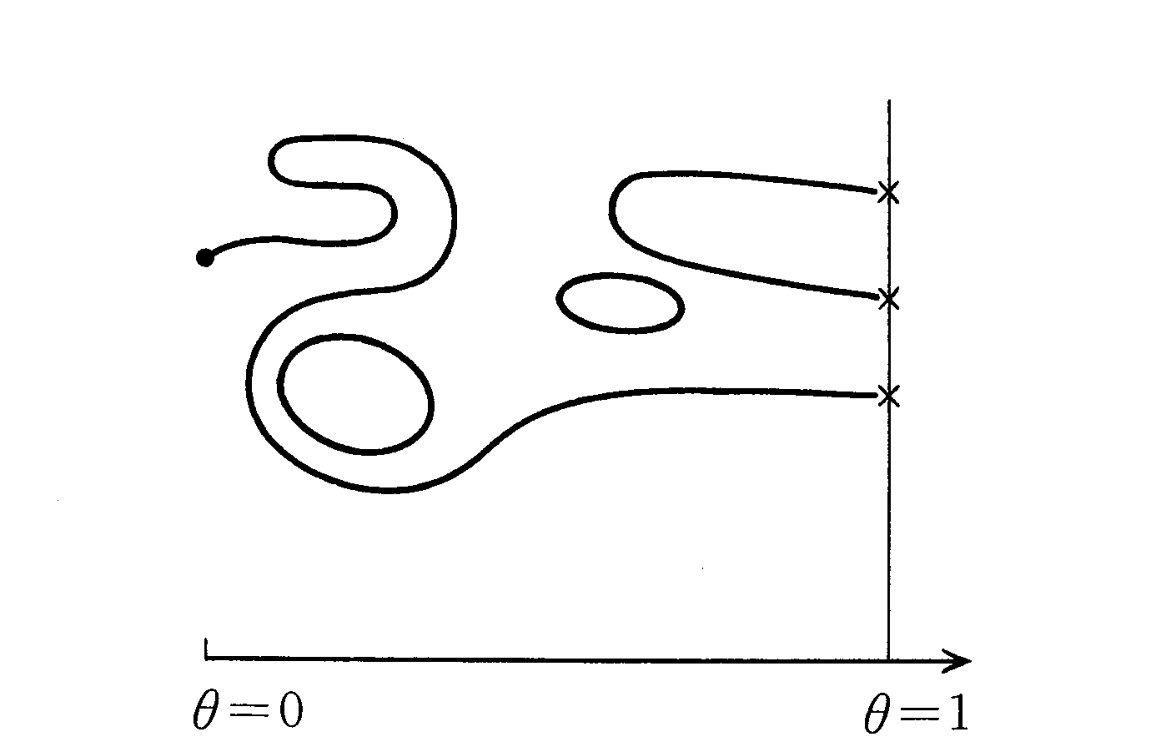
\includegraphics[width=0.62\textwidth]{figures/fig2.1.png}
  \figtitle{2.1}{连续法下的解的构成（原书 p.41）}
\end{figure}
% [Tutor Note: 图 2.1 画的是 $\mathcal{M}=\bigcup_\theta\mathcal{M}_\theta$：竖轴为 $\theta$，横轴为解；当 $\mathcal{M}$ 是一维带边流形且边界恰为 $\mathcal{M}_0\cup\mathcal{M}_1$ 时，$\theta=0$ 处的唯一解沿着一维轨道连到 $\theta=1$，故解必存在。]

命题 2.38 的证明的基本工具是 Atiyah–Singer 指数定理与隐函数定理。讨论的大部分对一般近凯勒流形 $(M,\omega_M,J_M)$ 的伪全纯映射也成立，故以下暂时考虑一般情形。取定一个 $\beta\in H_2(M;\Z)$。以 $\operatorname{Map}(S^2,M)$ 表示光滑映射 $\varphi\colon S^2\to M$ 全体。其部分集合 $\mathcal{X}$ 定义为
\[
  \mathcal{X}=\{\varphi\in\operatorname{Map}(S^2,M)\mid\varphi_*[S^2]=\beta\}.
\]
设 $\mathcal{E}$ 为 $\operatorname{Map}(S^2,M)$ 上的向量丛，其在 $\varphi$ 处的纤维为
\[
  \Gamma(S^2;\Lambda^{0,1}S^2\otimes_\C\varphi^*T^{1,0}M).
\]
这里 $\Lambda^{0,1}S^2$ 是 $S^2=\CP^1$ 上由 $0,1$ 形式构成的向量丛，$\varphi^*T^{1,0}M$ 是 $T^{1,0}M$ 经 $\varphi$ 拉回的向量丛。$\Gamma$ 指光滑截面全体。（$\varphi$ 变动时这些向量空间连续变动、确定向量丛，这一点容易证明。）

考虑 $M$ 的与 $\omega_M$ 相容的近复结构族 $J^\theta_M$。（分解 $TM\otimes\C=T^{1,0}M\oplus T^{0,1}M$ 依赖于 $\theta$，但 $T^{1,0}M$ 作为复向量丛的同构类在近复结构的连续形变下不变。因此可以认为 $\mathcal{E}$ 对任何 $\theta$ 的值都是同一个。）

% [原文 p.42]
$\Lambda^{0,1}S^2\otimes_\C\varphi^*T^{1,0}M$ 的截面可等同于反复线性映射 $TS^2\to\varphi^*(TM,J^\theta_M)$。又，$\varphi$ 的微分 $\rd\varphi$ 确定实线性映射 $TS^2\to\varphi^*(TM,J^\theta_M)$。把 $\rd\varphi$ 分成复线性部分与反复线性部分，把反复线性部分记为 $\bar\partial_\theta\varphi$，定义
\[
  s_\theta(\varphi)=\bar\partial_\theta\varphi.
\]
于是，$s_\theta(\varphi)=0$ 与 $\varphi$ 是（关于近复结构 $J^\theta_M$ 的）伪全纯映射，显然等价。由以上考察，我们就构成了以下各项。
\begin{enumerate}[label=(\arabic*),leftmargin=2.6em,itemsep=1pt,topsep=2pt]
  \item 无限维空间 $\mathcal{X}$；
  \item 其上的无限维向量丛 $\mathcal{E}$；
  \item $\mathcal{E}$ 的截面 $s_\theta$。
\end{enumerate}
而我们要研究的模空间就表为 $\mathcal{M}_\theta=s_\theta^{-1}(0)$。

把模空间表为“无限维空间上无限维向量丛的截面的零点集”，这是用几何学处理非线性偏微分方程时常见的想法。被称为拓扑场论（topological field theory）的理论大多是这样构成的。最初有组织地进行这种构造的，是规范理论（gauge theory），即自对偶（self-dual，或称 Yang–Mills）方程的情形。

像这样，把作为无限维向量丛截面的零点集而得到的模空间的基本同调类变成深刻的不变量——这是 Donaldson 在规范理论情形下发现的重要想法。Gromov 看穿了这一想法对辛流形的伪全纯曲线也适用。如前所述，得到辛流形不变量的重要方法是：找出由近复结构确定的量中对近复结构的连续形变不变者。在我们的情形，这意味着 $\mathcal{M}_\theta$ 的基本同调类不依赖 $\theta$。$\mathcal{M}_\theta$ 是 0 维的，故基本同调类就是“计及集合 $\mathcal{M}_\theta$ 的符号所得的个数”。也就是说，“计及 $\mathcal{M}_\theta$ 的符号所得的个数”不依赖 $\theta$，这就是中心主张。

% [原文 p.43]
模空间的基本同调类得以确定、并且在（定义模空间的方程的）连续形变下不变，这并不是任何时候都成立的。下面来看它成立的条件。

第 1 个条件是 Fredholm 性。为把问题点弄清，先作抽象化的讨论。回顾一下定义。

\begin{definition}{2.40}
  设 $\mathcal{E},\mathcal{F}$ 为 Banach 空间，线性映射 $\psi\colon\mathcal{E}\to\mathcal{F}$ 是\textbf{Fredholm 算子}（Fredholm operator），是指其核 $\Ker\psi=\{x\in\mathcal{E}\mid\psi x=0\}$ 与余核 $\Coker\psi=\mathcal{F}/\psi(\mathcal{E})$ 都是有限维的。

  $\dim\Ker\psi-\dim\Coker\psi$ 称为 $\psi$ 的\textbf{指数}（index）。

  Banach 流形 $X,Y$ 之间的可微映射 $\Psi\colon X\to Y$ 是\textbf{Fredholm 映射}（Fredholm map），是指它在各点的微分都是 Fredholm 算子。
\end{definition}

关于 Fredholm 算子在大范围分析与几何学中的意义、应用，在《指数定理》[135] 中有详述，请参阅。

Fredholm 算子的指数在算子的连续形变下不变（参见 [135]）。利用这一点，可以定义 Fredholm 映射 $\Psi\colon X\to Y$ 的指数。设 $X$ 连通。此时 $\Psi$ 在 $p\in X$ 处的微分 $\rd_p\Psi\colon T_pX\to T_{\Psi(p)}Y$ 的指数不依赖 $p$。称之为 $\Psi$ 的\textbf{指数}。

再稍作定义。下面的定义是有限维流形情形的定义的原样推广。

\begin{definition}{2.41}
  设 $\Psi\colon X\to Y$ 为 Banach 流形之间的可微映射。$p\in X$ 是\textbf{正则点}（regular point），是指微分 $\rd_p\Psi\colon T_pX\to T_{\Psi(p)}Y$ 是满射。$q\in Y$ 是\textbf{正则值}（regular value），是指 $\Psi^{-1}(q)$ 的所有点都是正则点。不是正则点的点称为\textbf{临界点}（critical point），不是正则值的点称为\textbf{临界值}（critical value）。
\end{definition}

下面的引理是 Banach 空间中隐函数定理的直接推论。

\begin{lemma}{2.42}
  若 $q\in Y$ 是指数为 $n$ 的 Fredholm 映射 $\Psi\colon X\to Y$ 的正则值，则 $\Psi^{-1}(q)$ 是 $n$ 维子流形。
\end{lemma}

% [原文 p.44]
下面的引理 2.43 是 Sard 定理（参见 [1]、[356] 等）的无限维化，属于 Smale [342]。证明从略。

\begin{lemma}{2.43}
  Fredholm 映射 $\Psi\colon X\to Y$ 的正则值全体所成集合在 $Y$ 中稠密。
\end{lemma}

Fredholm 映射 $\Psi$ 的指数，称为 $\Psi^{-1}(q)$ 的\textbf{虚拟维数}（virtual dimension）。

这里作一个简化假设。即设映射 $\Psi\colon X\to Y$ 是固有（proper）的。（这意味着任意紧集 $K\subset X$ 的逆像 $\Psi^{-1}(K)$ 是紧的。）（这相当于命题 2.39。）

现在设 $q_1,q_2$ 为 Fredholm 映射 $\Psi\colon X\to Y$ 的正则值。由引理 2.42，$\Psi^{-1}(q_1)$、$\Psi^{-1}(q_2)$ 是 $n$ 维紧子流形（$n$ 是 $\Psi$ 的指数）。假设 $Y$ 连通。

\begin{proposition}{2.44}
  $\Psi^{-1}(q_1)$ 的基本同调类 $[\Psi^{-1}(q_1)]\in H_n(X;\Z_2)$ 等于 $\Psi^{-1}(q_2)$ 的基本同调类 $[\Psi^{-1}(q_2)]\in H_n(X;\Z_2)$。
\end{proposition}

无限维空间之间的映射 $\Psi\colon X\to Y$ 中重要的是微分算子。此时 $\Psi^{-1}(q_1)$、$\Psi^{-1}(q_2)$ 是微分方程的解所成空间，即模空间。于是，命题 2.44 意味着模空间的基本同调类在方程连续变动时不变。

命题 2.44 在 $X,Y$ 有限维时是显然的。即 $[\Psi^{-1}(q_1)]$ 是 $\Psi^*([Y])$ 的 Poincaré 对偶（$[Y]\in H^{\dim Y}(Y;\Z_2)$ 是基本上同调类）。

在我们关心的情形，$X,Y$ 是无限维的，故基本上同调类 $[Y]$ 没有意义，上述论证不适用。但是，不把上同调群之类的概念装置摆到台面上，直接重新审视论证，便可如下证明命题 2.44。

取连接 $q_1$ 与 $q_2$ 的 $Y$ 的光滑道路 $\gamma\colon[0,1]\to Y$（$\gamma(0)=q_1$，$\gamma(1)=q_2$）。用它来考虑纤维积
\[
  X\times_Y[0,1]=\{(x,\tau)\in X\times[0,1]\mid\Psi(x)=\gamma(\tau)\}.
\]
下面的 2 个引理是引理 2.42 与 2.43 的推广。

% [原文 p.45]
\begin{lemma}{2.45}
  若对任意 $(x,\tau)\in X\times_Y[0,1]$，$\operatorname{Im}\rd_x\Psi$ 与 $\dfrac{\rd\gamma}{\rd\tau}$ 张成 $T_{\Psi(x)}Y$，则 $X\times_Y[0,1]$ 是 $n+1$ 维流形，且其边界 $\partial(X\times_Y[0,1])$ 是 $\Psi^{-1}(q_1)\cup\Psi^{-1}(q_2)$。
\end{lemma}

引理 2.45 可由隐函数定理得到。

\begin{lemma*}{2.46}
  若 $q_1,q_2$ 是正则值，则满足引理 2.45 的假设的道路 $\gamma$ 的集合，在连接 $q_1$ 与 $q_2$ 的道路全体所成集合中稠密。
\end{lemma*}

\begin{proof}[略证]
  把 $\gamma\colon[0,1]\to Y$、$\gamma(0)=q_1$、$\gamma(1)=q_2$ 这样的道路全体记为 $\mathcal{P}_Y$。令
  \[
    \mathcal{P}_X=\{(\gamma,x,\tau)\in\mathcal{P}_Y\times X\times[0,1]\mid\gamma(\tau)=\Psi(x)\}.
  \]
  $\mathcal{P}_Y,\mathcal{P}_X$ 是（无限维）流形\footnote{这里没有触及所考虑道路的光滑性以及道路空间的拓扑。由于想考虑由光滑道路构成的空间，按通常取法会成为 Fréchet 流形，而不是 Banach 流形。这对应用隐函数定理等不便。要么先在 $C^k$ 级的范围内讨论，最后用某种方法证明道路的光滑性，要么用 Floer 的技巧（[102] §5）作出由光滑道路构成的 Banach 流形。}，设 $\pi\colon\mathcal{P}_X\to\mathcal{P}_Y$ 为 $(\gamma,x,\tau)\mapsto\gamma$，则 $\pi$ 是 Fredholm 映射。故由引理 2.43，正则值在 $\mathcal{P}_Y$ 中稠密。$\pi$ 的正则值所对应的 $\mathcal{P}_Y$ 的元素满足引理 2.46 的结论。
\end{proof}

由这 2 个引理，命题 2.44 立即可得。

命题 2.44 所述的是证明结构最易看清、论证最简洁的情形。实际上，能由这个命题立即证明“模空间的基本同调类在方程形变下不变”的情形并不多。（由单极子方程（monopole equation）决定的 4 维流形的不变量 Seiberg–Witten 不变量（Seiberg-Witten invariant），是几乎只需这些就足够的例子。）

回到伪全纯曲线的模空间。要应用此前的讨论，首先必须考虑的不是光滑映射的范畴，而是其完备化。（光滑映射全体不是 Banach 空间而是 Fréchet 空间，在其上考虑隐函数定理等更困难。）这可以通过考虑适当的 Sobolev 空间（Sobolev space）而成为可能。本节不涉及这一点。（参见定义 5.50。）

% [原文 p.46]
我们的情形不是无限维流形之间有映射，而是无限维流形 $\mathcal{X}$ 上的向量丛 $\mathcal{E}$ 及其截面。此时应如何把“Fredholm 映射”的概念推广为“Fredholm 截面”呢？为此，考虑向量丛在一点 $p\in\mathcal{X}$ 附近的平凡化 $\mathcal{E}|_{U_p}\simeq U_p\times\mathcal{E}_p$，把截面 $s\colon\mathcal{X}\to\mathcal{E}$ 局部地看成映射 $s_p\colon U_p\to\mathcal{E}_p$ 即可（即 $s(x)=(x,s_p(x))$）。若对任意 $p$，$s_p$ 在 $p$ 处的微分都是 Fredholm 算子，就称 $s$ 为\textbf{Fredholm 截面}。

在几乎所有重要的例子里，$s$ 是非线性微分算子，其微分 $\rd_ps$ 是线性微分算子。这种情形下，线性微分方程 $\rd_ps=0$ 称为 $s=0$ 的\textbf{线性化方程}（linearized equation）。

\begin{remark}{2.47}
  上面所述 Fredholm 截面的定义有一个问题。即“Fredholm 截面”这一概念是否依赖于局部平凡化，并不清楚。考虑完全一般的 Banach 流形及其上的 Banach 向量丛时，这看来是不正确的。不过，当 $s(p)=0$ 时，有标准分解 $T_{(p,0)}\mathcal{E}=T_pX\oplus\mathcal{E}_p$。用它，线性映射 $\rd_ps\colon T_pX\to\mathcal{E}_p$ 可不依赖局部平凡化地确定。因此，“在 $s(p)=0$ 的点处 $s$ 的微分是 Fredholm 算子”这一陈述有不依赖局部平凡化的意义。

  但是，仿照命题 2.44 去证明 $s$ 的零点集的基本同调类在 $s$ 的连续形变下不变，仅假设 $s(p)=0$ 处具有 Fredholm 性恐怕不够。把这一点变得可能的抽象框架，本书不去尝试。

  在我们的情形，取如下的局部平凡化即可。给定 $\varphi$ 时，对与 $\varphi$ 充分接近的 $\varphi'$，如下确定纤维 $\Gamma(S^2;\Lambda^{0,1}S^2\otimes_\C\varphi^*T^{1,0}M)$ 与 $\Gamma(S^2;\Lambda^{0,1}S^2\otimes_\C\varphi'^*T^{1,0}M)$ 之间、随 $\varphi'$ 变动而光滑变动的同构：对 $x\in S^2$，用 $\varphi(x)$ 与 $\varphi'(x)$ 之间的最短测地线作平行移动，确定 $\varphi^*TM$ 与 $\varphi'^*TM$ 之间的同构；再取其复线性成分，得到 $\varphi^*T^{1,0}M$ 与 $\varphi'^*T^{1,0}M$ 之间的同构即可（[124] §12）。

  当然还有其他各种取法，但若不回到有限维的状况去定义，多半会出问题。在抽象的无限维流形论框架内去构造，就会越来越危险。本节之所以使用无限维流形，只是为了便于理解的权宜之计；把一般的无限维几何学抽象地展开、再作为其推论来论述各种事情，似乎还不到那样的阶段。
\end{remark}

% [原文 p.47]
那么，我们的截面 $s_\theta(\varphi)=\bar\partial_\theta\varphi$ 是 Fredholm 截面吗？这一点首先与我们所考虑的是从复 1 维流形出发的映射空间有关。为看清这一点，来计算 $s_\theta$ 在满足 $s_\theta(\varphi)=0$ 的 $\varphi$ 处的微分。（如注意 2.47 所述，这不依赖局部平凡化而有意义。）

无限维流形 $\operatorname{Map}(S^2,M)$ 在一点 $\varphi$ 处的切空间是 $\Gamma(S^2;\varphi^*TM)$。这可以如下确认。设 $\gamma\colon(-\varepsilon,\varepsilon)\to\operatorname{Map}(S^2,M)$ 为满足 $\gamma(0)=\varphi$ 的光滑曲线。即 $\gamma(\tau)$ 是 $S^2\to M$ 的曲线。于是，对每个 $x\in S^2$，$\rd(\gamma(\tau)(x))/\rd\tau$ 在 $\tau=0$ 处的值是切向量 $\in T_{\varphi(x)}M$。因此确定 $\Gamma(S^2;\varphi^*T(S^2\times S^2))$ 的元素。把它看作 $\gamma$ 在原点处的切向量。
% [Tutor Note: 原书 p.47 此处作“$\Gamma(S^2;\varphi^*T(S^2\times S^2))$”，但按上一句“切向量 $\in T_{\varphi(x)}M$”，应读作 $\Gamma(S^2;\varphi^*TM)$；原书疑有笔误。正文照录。]

现在设 $\varphi\colon S^2\to M$ 为关于 $J^\theta_M$ 的伪全纯曲线，$V\in\Gamma(S^2;\varphi^*TM)$。来计算截面 $s_\theta$ 在 $\varphi$ 处的微分 $\rd_\varphi s_\theta$ 在 $V$ 处的值 $\in\Gamma(S^2;\Lambda^{0,1}\otimes\varphi^*TM)$。计算它在 $w_0\in S^2$ 处的值。令 $p=\varphi(w_0)$，选取 $p$ 附近 $M$ 的坐标 $z_1,\dots,z_m$（$z_i=x_i+\sqrt{-1}\,y_i$），使 $\rd z_1,\dots,\rd z_m$ 成为 $\Lambda_p^{1,0}M$ 的基。由于 $J^\theta_M$ 不可积，不能在各点都使 $\rd z_1,\dots,\rd z_m$ 含于 $\Lambda^{1,0}M$；在一点上则可以。

令
\[
  V(w)=\sum a_i(w)\frac{\partial}{\partial x_i}+b_i(w)\frac{\partial}{\partial y_i}.
\]
曲线 $\gamma\colon(-\varepsilon,\varepsilon)\to\operatorname{Map}(S^2,M)$ 定义为
\[
  \gamma(\tau)(w)_i=\varphi(w)_i+\tau a_i(w)+\sqrt{-1}\,\tau b_i(w).
\]
（$\varphi(w)_i$ 表示 $\varphi(w)$ 的 $z_i$ 坐标，$\gamma(\tau)(w)_i$ 表示 $\gamma(\tau)(w)$ 的 $z_i$ 坐标。）$\gamma$ 在原点处的切向量就是 $V$。

% [原文 p.48]
引入 $w_0$ 附近的 $S^2$ 的复坐标 $w=s+\sqrt{-1}\,t$。想计算 $(\bar\partial_\theta\gamma(\tau))(w_0)$ 的 $\tau$ 微分在 $\tau=0$ 处的值。设 $w_0=0$ 不失一般性。把 $w$ 映到 $(\tau a_1(w)+\sqrt{-1}\tau b_1(w),\ a_1(w)+\sqrt{-1}b_1(w))$ 的映射记为 $V(w)\colon D(\varepsilon)\to\C^2$（$D(\varepsilon)$ 是 $\C$ 中半径为 $\varepsilon$ 的圆盘）。

$(\bar\partial_\theta\gamma(\tau))(0)$ 是 $V(w)$ 的微分（Jacobi 矩阵）$\rd_0V$ 关于 $J^\theta_{\gamma(\tau)(w)}$ 的反复线性成分。设 $\Pi_\tau\colon\Hom(\R^2,\R^{2m})\to\operatorname{AntiHom}(\C,\C^m)$ 为到关于 $J^\theta_{\gamma(\tau)(w)}$ 的反复线性成分的投影。又，以 $\bar\partial V(u_0)$ 表示 $\rd_0V$ 关于 $J^0$（即通常的复结构）的反复线性成分。于是，$(\bar\partial_\theta\gamma(\tau))(0)$ 的 $\tau$ 微分在 $\tau=0$ 处的值是
\begin{equation}
  \bar\partial V(0)+\frac{\partial\Pi_\tau}{\partial\tau}\rd u_0 \tag{2.19}
\end{equation}
应当注意的是，第 2 项不含关于 $V$ 的微分；也就是说，第 2 项是 0 阶微分算子。第 1 项是 1 阶微分算子。

以上的计算表为
\begin{equation}
  (\rd_\varphi s)(V)=\bar\partial V+\mathcal{N}'(V) \tag{2.20}
\end{equation}
这里 $\mathcal{N}'$ 是 0 阶微分算子。(2.20)$\,=0$ 是 $\bar\partial_\theta\varphi=0$ 的线性化方程。

\begin{remark}{2.48}
  如果近复结构 $J^\theta$ 是复结构，那么上面的计算可以使用复坐标 $z_i$。此时 $J^\theta$ 在每一点都是通常的 $\sqrt{-1}$ 倍，故 $\Pi_\tau$ 不依赖 $\tau$。即 (2.20) 的第 2 项为 0。因此第 2 项可用 $\mathcal{N}$ 表示。在 (2.20) 中写作 $\mathcal{N}'$，是因为这一项由 $\mathcal{N}$ 确定，但它并不是 $\mathcal{N}$ 本身。
\end{remark}

为弄清 (2.20) 的第 1 项 $\bar\partial V$ 在 $S^2$ 上的整体意义，简单复习正则向量丛与以其为系数的 Dolbeault 复形。详见 [206]。

复流形 $M$ 上的复向量丛 $\pi\colon E\to M$ 是\textbf{正纯向量丛}（holomorphic vector bundle），是指存在开覆盖 $M=\bigcup U_i$ 与向量丛的局部平凡化 $\varphi_i\colon\pi^{-1}U_i\simeq$

% [原文 p.49]
$U_i\times\C^n$，使得按 $g_{ij}(x)(v)=\varphi_i\varphi_j^{-1}(x,v)$ 定义的 $g_{ij}\colon U_i\cap U_j\to GL(n;\C)$ 为正纯函数。这样的 $U_i,\varphi_i$ 称为正纯的平凡化。

考虑正纯向量丛 $\pi\colon E\to M$ 的截面 $s$。用正纯平凡化 $U_i,\varphi_i$，定义 $s_i\colon U_i\to\C^n$ 为 $(x,s_i(x))=\varphi_is(x)$。由 $g_{ij}$ 正纯可知 $g_{ij}\bar\partial s_j=\bar\partial s_i$。故 $s_i$ 相互贴合，确定 $E\otimes\Lambda^{0,1}M$ 的截面。记之为 $\bar\partial s$。

以上确定了映射 $\bar\partial\colon\Gamma(E)\to\Gamma(E\otimes\Lambda^{0,1}M)$。它可扩充为 $\bar\partial\colon\Gamma(E\otimes\Lambda^{0,k}M)\to\Gamma(E\otimes\Lambda^{0,k+1}M)$（参见 [206]）。于是得到 $E$ 系数的 Dolbeault 复形。下面的定理是定理 2.35 的类似。

\begin{theorem}{2.49}
  下面 2 个条件等价。
  \begin{enumerate}[label=(\arabic*),leftmargin=2.2em,itemsep=1pt,topsep=2pt]
    \item $E$ 是正纯向量丛。
    \item 存在 $\bar\partial\colon\Gamma(E\otimes\Lambda^{0,k}M)\to\Gamma(E\otimes\Lambda^{0,k+1}M)$，使得对 $u\in\Gamma(E\otimes\Lambda^{0,k}M)$、$v\in\Gamma(\Lambda^{0,l}M)$ 满足
    \[
      \bar\partial\bar\partial=0,\qquad \bar\partial(u\wedge v)=\bar\partial u\wedge v+(-1)^{\deg u}u\wedge\bar\partial v.
    \]
  \end{enumerate}
\end{theorem}

\begin{proof}[略证]
  (1)$\Rightarrow$(2) 已说明。逆的证明与定理 2.35 的证明相近。即假设 (2)，在各点 $p$ 的邻域寻找 $\bar\partial s_k=0$ 的 $s_k$（$k=1,\dots,n$），使 $s_1(p),\dots,s_n(p)$ 成为 $E_p$ 的基。（于是 $u=\sum u_ks_k\mapsto(u_1,\dots,u_n)$ 给出 $p$ 的邻域上的正纯平凡化。）保证方程 $\bar\partial s=0$ 可解的条件是 $\bar\partial\bar\partial=0$。详见 [79] §2.1。
\end{proof}

\begin{corollary}{2.50}
  复 1 维流形（黎曼面）上的任意复向量丛都具有正纯向量丛的结构。
\end{corollary}

这由 $\bar\partial\bar\partial=0$ 在黎曼面情形自动成立可得。

\begin{lemma*}{2.51}
  设 $\bar\partial^1$、$\bar\partial^2$ 为同一复向量丛的两个不同正纯向量丛结构所确定的 Dolbeault 算子。此时 $\bar\partial^1-\bar\partial^2$ 是 0 阶微分算子。
\end{lemma*}

\begin{proof}
  由定理 2.49(2) 的第 2 个条件式，$\bar\partial^i(fu)=\bar\partial f\wedge u+f\bar\partial^iu$ 成立。故 $(\bar\partial^2-\bar\partial^1)(fu)=f(\bar\partial^2-\bar\partial^1)(u)$。即 $\bar\partial^1-\bar\partial^2$ 是 0 阶微分算子。
\end{proof}

% [原文 p.50]
以上结束了关于正纯向量丛的复习。来给 (2.25) 的第 1 项赋予整体意义。
% [Tutor Note: 原书 p.50 此处作“式 (2.25)”，但下文讨论的“第 1 项 $\bar\partial V$”出自 (2.20)，(2.25) 是下一节的编号，疑为笔误，应为 (2.20)。正文照录。]

设 $\varphi\colon S^2\to M$ 为伪全纯映射。$\varphi^*T^{1,0}M$ 是复向量丛。由推论 2.50，它具有正纯向量丛的结构。固定其中一种。

\begin{lemma}{2.52}
  $V\mapsto\rd_\varphi s(V)-\bar\partial V$ 是 0 阶微分算子。
\end{lemma}

除 0 阶微分算子外，$\bar\partial$ 不依赖正纯向量丛的结构。注意到这一点，由已经做过的计算，证明是显然的。

\begin{remark}{2.53}
  推论 2.50 并非引理 2.52 的证明所必需（即使 $\varphi^*T^{1,0}M$ 上没有正纯向量丛结构，$\bar\partial V$ 仍有意义）。因此，$S^2$ 是复 1 维这一点，本质上被用到的地方并非此处。
\end{remark}

$S^2$ 是复 1 维这一点，本质上被用到的地方是下面的引理。

\begin{lemma}{2.54}
  设 $\Sigma$ 为黎曼面，$E\to\Sigma$ 为正纯向量丛，则 $\bar\partial\colon\Gamma(E)\to\Gamma(E\otimes\Lambda^{0,1})$ 是 Fredholm 算子。
\end{lemma}

这是关于 Dolbeault 复形的下述著名定理的推论。

\begin{theorem}{2.55}
  $\bar\partial$ 确定椭圆型复形 $E\to E\otimes\Lambda^{0,1}\to E\otimes\Lambda^{0,2}\to\cdots\to E\otimes\Lambda^{0,n}$（$n$ 是 $M$ 的复维数）。
\end{theorem}

椭圆型复形的定义及定理 2.55 的证明请参阅 [135]，此处从略。

\begin{proof}[引理 2.54 的证明]
  黎曼面情形下，由定理 2.55，长度为 2 的复形 $\bar\partial\colon E\to E\otimes\Lambda^{0,1}$ 是椭圆型复形。这意味着 $\bar\partial$ 是椭圆型微分算子。因此，如所周知（例如参见 [135]），$\bar\partial\colon\Gamma(E)\to\Gamma(E\otimes\Lambda^{0,1})$ 是 Fredholm 算子。
\end{proof}

引理 2.54 的证明中，我们证明了 $\bar\partial$ 是 1 阶椭圆型算子。这一性质在加上 0 阶微分算子后不变。因此，由引理 2.51，$\rd_\varphi s_\theta(V)$ 也是椭圆型的。于是得到了下面的事实。

\begin{theorem}{2.56}
  设 $\varphi\colon S^2\to M$ 为伪全纯映射，则微分算子 $\rd_\varphi s_\theta\colon\Gamma(\varphi^*TM)\to\Gamma(\varphi^*TM\otimes\Lambda^{0,1})$ 是 Fredholm 算子。
\end{theorem}

% [原文 p.51]
这里，若考虑的不是复 1 维空间 $S^2$，而是从更高维空间出发的映射，则定理 2.56 不再成立；这一点先看清楚。例如设 $\varphi\colon\CP^2\to\CP^3$ 为伪全纯映射。（$\CP^3$ 上取不可积的近复结构，$\CP^2$ 上取通常的复结构。）此时复向量丛 $\varphi^*T^{1,0}\CP^3$ 一般没有正纯结构，故以它为系数的 Dolbeault“复形”本来就不是复形（$\bar\partial\bar\partial=0$ 不成立）。暂且对这一点视而不见，假设 $\varphi^*T^{1,0}\CP^3$ 上有正纯结构。然而此时 Dolbeault 复形是
\[
  \varphi^*T^{1,0}\CP^3\to\varphi^*T^{1,0}\CP^3\otimes\Lambda^{0,1}\to\varphi^*T^{1,0}\CP^3\otimes\Lambda^{0,2},
\]
故只考虑 $\varphi^*T^{1,0}\CP^3\to\varphi^*T^{1,0}\CP^3\otimes\Lambda^{0,1}$ 并非椭圆型。换言之，上同调
\[
  \frac{\Ker\bar\partial\colon\Gamma(\varphi^*T^{1,0}\CP^3\otimes\Lambda^{0,1})\to\Gamma(\varphi^*T^{1,0}\CP^3\otimes\Lambda^{0,2})}{\operatorname{Im}\bar\partial\colon\Gamma(\varphi^*T^{1,0}\CP^3)\to\Gamma(\varphi^*T^{1,0}\CP^3\otimes\Lambda^{0,1})}
\]
是有限维的，而
\[
  \Coker\bar\partial\colon\Gamma(\varphi^*T^{1,0}\CP^3)\to\Gamma(\varphi^*T^{1,0}\CP^3\otimes\Lambda^{0,1})
\]
是无限维的。也就是说，映射
\[
  \bar\partial\colon\Gamma(\varphi^*T^{1,0}\CP^3)\to\Gamma(\varphi^*T^{1,0}\CP^3\otimes\Lambda^{0,1})
\]
的指数是 $-\infty$。这意味着 $\CP^2\to\CP^3$ 的伪全纯映射的模空间的虚拟维数是 $-\infty$。

这一点在前一节也已述及。那里所述的理由是 $\CP^2$ 上的近复结构一般不可积，而这归结为 $\Lambda^{0,2}\CP^2$ 不为 0。$\bar\partial$ 不成为 Fredholm 算子也是同一理由。当然这一致并非偶然，只不过是同一件事的不同侧面而已。

回到黎曼面的情形。由定理 2.56，$\rd_\varphi s_\theta$ 是 Fredholm 算子。其指数用 Riemann–Roch 定理计算如下。

\begin{theorem}{2.57}
  设 $E$ 为亏格 $g$ 的闭黎曼面 $\Sigma$ 上的正纯向量丛，$c^1(E)$ 为其第 1 Chern 类。此时 Dolbeault 算子 $\bar\partial\colon\Gamma(E)\to\Gamma(E\otimes\Lambda^{0,1})$ 的指数 $\operatorname{Index}\bar\partial$ 由下式给出。
  \[
    \operatorname{Index}\bar\partial=(2-2g)\operatorname{rank}_\C E+2[\Sigma]\cap c^1(E).
  \]
\end{theorem}

% [原文 p.52]
定理的证明从略。参见 [135]。

$\rd_\varphi s_\theta$ 与 $\bar\partial$ 只相差 0 阶算子。由 Fredholm 算子指数的连续形变性，$\rd_\varphi s_\theta$ 的指数与 $\bar\partial$ 的指数一致。于是 $\rd_\varphi s_\theta$ 的指数就算出来了。

现在，定理 2.36 中出现的是定理 2.57 中 $S^2$ 上正纯向量丛 $\varphi^*T^{1,0}\CP^2$ 的情形。即 $g=0$、$\operatorname{rank}_\C E=2$。又 $\varphi_*[S^2]=[\CP^1]$。故由 $c^1(T^{1,0}\CP^2)=3[\CP^1]$ 得
\[
  \int_{S^2}c^1(\varphi^*T^{1,0}\CP^2)=3.
\]
因此得到 $\operatorname{Index}\rd_\varphi s_\theta=10$。

然而，上面的计算考虑的是 $\operatorname{Map}(S^2,\CP^2)$，也就是说没有考虑 $\varphi(0)\in\CP^1$、$\varphi(1)=[1:0:1]$、$\varphi(\infty)=[0:1:1]$ 这些条件。因此要计算模空间 $\mathcal{M}_\theta$ 的维数，必须从中减去 $4\times2+2=10$。于是维数为 0。也就是说，若前面关于 Fredholm 映射所说明的引理 2.42 与引理 2.43 之类的事实在我们的情形成立，则稍微变动 $s_\theta$，$\mathcal{M}_\theta=s_\theta^{-1}(0)$ 就成为 0 维流形。进一步，若引理 2.45、2.46 之类的事实成立，则 $\mathcal{M}=\bigcup\mathcal{M}_\theta$ 成为 1 维流形，其边界为 $\mathcal{M}_0\cup\mathcal{M}_1$。这就是命题 2.38 的主张。

\begin{remark}{2.58}
  引理 2.42、2.43、2.45、2.46 的状况比我们的状况简化了，由这些引理并不能直接推出命题 2.38。不过，比以上说明所必需的更多的东西，是隐函数定理与 Sobolev 不等式（Sobolev inequality）等，它们的使用方式也是一般的，故不再作更多说明。
\end{remark}

\begin{remark}{2.59}
  计算指数时，$\rd_\varphi s_\theta$ 与 $\bar\partial$ 之差 $\mathcal{N}'$（这是 $J^\theta_M$ 不可积的效果）并不重要；但 $\mathcal{N}'$ 并非任何时候都可以忽视。作为 $\mathcal{N}'$ 的效果，下面这一点很重要。$\Gamma(\varphi^*TM)$、$\Gamma(\varphi^*TM\otimes\Lambda^{0,1})$ 是复向量空间，$\bar\partial$ 是复线性的，但 $\mathcal{N}'$（从而 $\rd_\varphi s_\theta$）未必是复线性的。
\end{remark}

% CHUNK ch02a DONE
